\section{Numerical realization of the bisection}
\label{sec:numer-real-mount}

The procedure described in \ref{sec:bisection} can be easily realized
by solving the PDE \eqref{eq:en_flow} numerically. For $H_+$, we start
by choosing $g_+$ to be
\begin{align}
  \label{eq:98}
  g_+(\psi)=\pi\sin\psi.
\end{align}
Then, the proper $A^*$ is found by bisection between the blow-up and
the convergence to $0$. As the bisection cannot yield an exact value
of $A^*$ (due to the finite machine precision) we are not able to
reach precisely the saddle point. Rather, as we are starting a bit off
the mid-line between attractors, the solution slides along it reaching
the neighbourhood of $f_2$ along its stable direction, it stays put
for some time but then starts to move again, slowly decaying along the
unstable direction to finally either fall into $0$ or blow up. The
smaller the numerical error of $A^*$ the closer we get to the mid-line
and the longer solutions stays near $f_2$.\\

From the numerical solutions to PDE \eqref{eq:en_flow} we can read the
quantities involved in approaching and leaving the neighbourhood of
$f_2$. These are the first two modes of $f_2$ along with their
respective eigenvalues as presented in \eqref{eq:69}. To obtain the
eigenvalues $\lb{2}{0}$ and $\lb{2}{2}$ we use the function
$\partial_tf\big|_{r=\pi/2}$ which, while in a close neighbourhood of
$f_2$ is
\begin{align}
  \label{eq:99}
  \partial_t
  f\big|_{r=\pi/2}=-\lambda_0A_0e^{-\lambda_0t}v_0(\pi/2)-\lambda_2A_2e^{-\lambda_2t}v_2(\pi/2)
\end{align}
(we have dropped the upper index for clarity). $v_0(\pi/2)$ and
$v_2(\pi/2)$ are quantities depending on the normalization of our
choice, and to further simplify the calculations we set
\begin{align}
  \label{eq:100}
  v_{0,2}(\pi/2)=1.
\end{align}
The quantities $A_{0,2}$ and $\lb{2}{0,2}$ resulting from fitting the
function \eqref{eq:99} to its analog from numerically solved PDE along
with $A^*$ calculated from the bisection are presented in Table ???.\\

Figures ??? present the stages of the evolution.

% \begin{sideways}
%     \centering
%     \label{fig:Evol2}

% \hspace*{-1.5in}
\begin{figure}[h]
  \label{fig:snapshot2}
  \centering
  \advance\leftskip-3cm
  % GNUPLOT: LaTeX picture with Postscript
\begingroup
  \makeatletter
  \providecommand\color[2][]{%
    \GenericError{(gnuplot) \space\space\space\@spaces}{%
      Package color not loaded in conjunction with
      terminal option `colourtext'%
    }{See the gnuplot documentation for explanation.%
    }{Either use 'blacktext' in gnuplot or load the package
      color.sty in LaTeX.}%
    \renewcommand\color[2][]{}%
  }%
  \providecommand\includegraphics[2][]{%
    \GenericError{(gnuplot) \space\space\space\@spaces}{%
      Package graphicx or graphics not loaded%
    }{See the gnuplot documentation for explanation.%
    }{The gnuplot epslatex terminal needs graphicx.sty or graphics.sty.}%
    \renewcommand\includegraphics[2][]{}%
  }%
  \providecommand\rotatebox[2]{#2}%
  \@ifundefined{ifGPcolor}{%
    \newif\ifGPcolor
    \GPcolortrue
  }{}%
  \@ifundefined{ifGPblacktext}{%
    \newif\ifGPblacktext
    \GPblacktexttrue
  }{}%
  % define a \g@addto@macro without @ in the name:
  \let\gplgaddtomacro\g@addto@macro
  % define empty templates for all commands taking text:
  \gdef\gplbacktext{}%
  \gdef\gplfronttext{}%
  \makeatother
  \ifGPblacktext
    % no textcolor at all
    \def\colorrgb#1{}%
    \def\colorgray#1{}%
  \else
    % gray or color?
    \ifGPcolor
      \def\colorrgb#1{\color[rgb]{#1}}%
      \def\colorgray#1{\color[gray]{#1}}%
      \expandafter\def\csname LTw\endcsname{\color{white}}%
      \expandafter\def\csname LTb\endcsname{\color{black}}%
      \expandafter\def\csname LTa\endcsname{\color{black}}%
      \expandafter\def\csname LT0\endcsname{\color[rgb]{1,0,0}}%
      \expandafter\def\csname LT1\endcsname{\color[rgb]{0,1,0}}%
      \expandafter\def\csname LT2\endcsname{\color[rgb]{0,0,1}}%
      \expandafter\def\csname LT3\endcsname{\color[rgb]{1,0,1}}%
      \expandafter\def\csname LT4\endcsname{\color[rgb]{0,1,1}}%
      \expandafter\def\csname LT5\endcsname{\color[rgb]{1,1,0}}%
      \expandafter\def\csname LT6\endcsname{\color[rgb]{0,0,0}}%
      \expandafter\def\csname LT7\endcsname{\color[rgb]{1,0.3,0}}%
      \expandafter\def\csname LT8\endcsname{\color[rgb]{0.5,0.5,0.5}}%
    \else
      % gray
      \def\colorrgb#1{\color{black}}%
      \def\colorgray#1{\color[gray]{#1}}%
      \expandafter\def\csname LTw\endcsname{\color{white}}%
      \expandafter\def\csname LTb\endcsname{\color{black}}%
      \expandafter\def\csname LTa\endcsname{\color{black}}%
      \expandafter\def\csname LT0\endcsname{\color{black}}%
      \expandafter\def\csname LT1\endcsname{\color{black}}%
      \expandafter\def\csname LT2\endcsname{\color{black}}%
      \expandafter\def\csname LT3\endcsname{\color{black}}%
      \expandafter\def\csname LT4\endcsname{\color{black}}%
      \expandafter\def\csname LT5\endcsname{\color{black}}%
      \expandafter\def\csname LT6\endcsname{\color{black}}%
      \expandafter\def\csname LT7\endcsname{\color{black}}%
      \expandafter\def\csname LT8\endcsname{\color{black}}%
    \fi
  \fi
  \setlength{\unitlength}{0.0500bp}%
  \begin{picture}(10080.00,10080.00)%
      \csname LTb\endcsname%
      \put(5040,9860){\makebox(0,0){\strut{}Asymetric modes of $f_3$ and $f_1$}}%
    \gplgaddtomacro\gplbacktext{%
      \put(2889,6579){\makebox(0,0){\strut{}$t=0.0$}}%
    }%
    \gplgaddtomacro\gplfronttext{%
    }%
    \gplgaddtomacro\gplbacktext{%
      \csname LTb\endcsname%
      \put(2488,8534){\makebox(0,0)[r]{\strut{}$\pi/2$}}%
      \csname LTb\endcsname%
      \put(3157,7777){\makebox(0,0){\strut{}$\pi/2$}}%
    }%
    \gplgaddtomacro\gplfronttext{%
    }%
    \gplgaddtomacro\gplbacktext{%
      \csname LTb\endcsname%
      \put(5577,6579){\makebox(0,0){\strut{}$t=0.5$}}%
    }%
    \gplgaddtomacro\gplfronttext{%
    }%
    \gplgaddtomacro\gplbacktext{%
    }%
    \gplgaddtomacro\gplfronttext{%
    }%
    \gplgaddtomacro\gplbacktext{%
      \csname LTb\endcsname%
      \put(8264,6579){\makebox(0,0){\strut{}$t=1.0$}}%
    }%
    \gplgaddtomacro\gplfronttext{%
    }%
    \gplgaddtomacro\gplbacktext{%
    }%
    \gplgaddtomacro\gplfronttext{%
    }%
    \gplgaddtomacro\gplbacktext{%
      \csname LTb\endcsname%
      \put(2889,3891){\makebox(0,0){\strut{}$t=1.5$}}%
    }%
    \gplgaddtomacro\gplfronttext{%
    }%
    \gplgaddtomacro\gplbacktext{%
    }%
    \gplgaddtomacro\gplfronttext{%
    }%
    \gplgaddtomacro\gplbacktext{%
      \csname LTb\endcsname%
      \put(5577,3891){\makebox(0,0){\strut{}$t=2.0$}}%
    }%
    \gplgaddtomacro\gplfronttext{%
    }%
    \gplgaddtomacro\gplbacktext{%
    }%
    \gplgaddtomacro\gplfronttext{%
    }%
    \gplgaddtomacro\gplbacktext{%
      \csname LTb\endcsname%
      \put(8264,3891){\makebox(0,0){\strut{}$t=2.5$}}%
    }%
    \gplgaddtomacro\gplfronttext{%
    }%
    \gplgaddtomacro\gplbacktext{%
    }%
    \gplgaddtomacro\gplfronttext{%
    }%
    \gplgaddtomacro\gplbacktext{%
      \csname LTb\endcsname%
      \put(876,1008){\makebox(0,0)[r]{\strut{}$10^{-2}$}}%
      \put(876,1680){\makebox(0,0)[r]{\strut{}$10^{-1}$}}%
      \put(876,2351){\makebox(0,0)[r]{\strut{}$10^{0}$}}%
      \put(876,3023){\makebox(0,0)[r]{\strut{}$10^{1}$}}%
      \put(876,3695){\makebox(0,0)[r]{\strut{}$10^{2}$}}%
      \put(1008,788){\makebox(0,0){\strut{}$0$}}%
      \put(2352,788){\makebox(0,0){\strut{}$\pi/4$}}%
      \put(3696,788){\makebox(0,0){\strut{}$\pi/2$}}%
      \put(1008,788){\makebox(0,0){\strut{}}}%
      \put(2352,788){\makebox(0,0){\strut{}}}%
      \put(3696,788){\makebox(0,0){\strut{}}}%
      \put(-17,2351){\rotatebox{90}{\makebox(0,0){\strut{}$f_t(t,r)$}}}%
      \put(2352,458){\makebox(0,0){\strut{}$\psi$}}%
      \put(2889,1203){\makebox(0,0){\strut{}$t=3.0$}}%
    }%
    \gplgaddtomacro\gplfronttext{%
    }%
    \gplgaddtomacro\gplbacktext{%
    }%
    \gplgaddtomacro\gplfronttext{%
    }%
    \gplgaddtomacro\gplbacktext{%
      \csname LTb\endcsname%
      \put(5577,1203){\makebox(0,0){\strut{}$t=3.5$}}%
    }%
    \gplgaddtomacro\gplfronttext{%
    }%
    \gplgaddtomacro\gplbacktext{%
    }%
    \gplgaddtomacro\gplfronttext{%
    }%
    \gplgaddtomacro\gplbacktext{%
      \csname LTb\endcsname%
      \put(8264,1203){\makebox(0,0){\strut{}$t=4.0$}}%
      \put(7190,3158){\makebox(0,0)[l]{\strut{}$\vn{1}{3}$}}%
      \put(6652,2674){\makebox(0,0)[l]{\strut{}$\vn{3}{3}$}}%
    }%
    \gplgaddtomacro\gplfronttext{%
    }%
    \gplgaddtomacro\gplbacktext{%
    }%
    \gplgaddtomacro\gplfronttext{%
    }%
    \gplbacktext
    \put(0,0){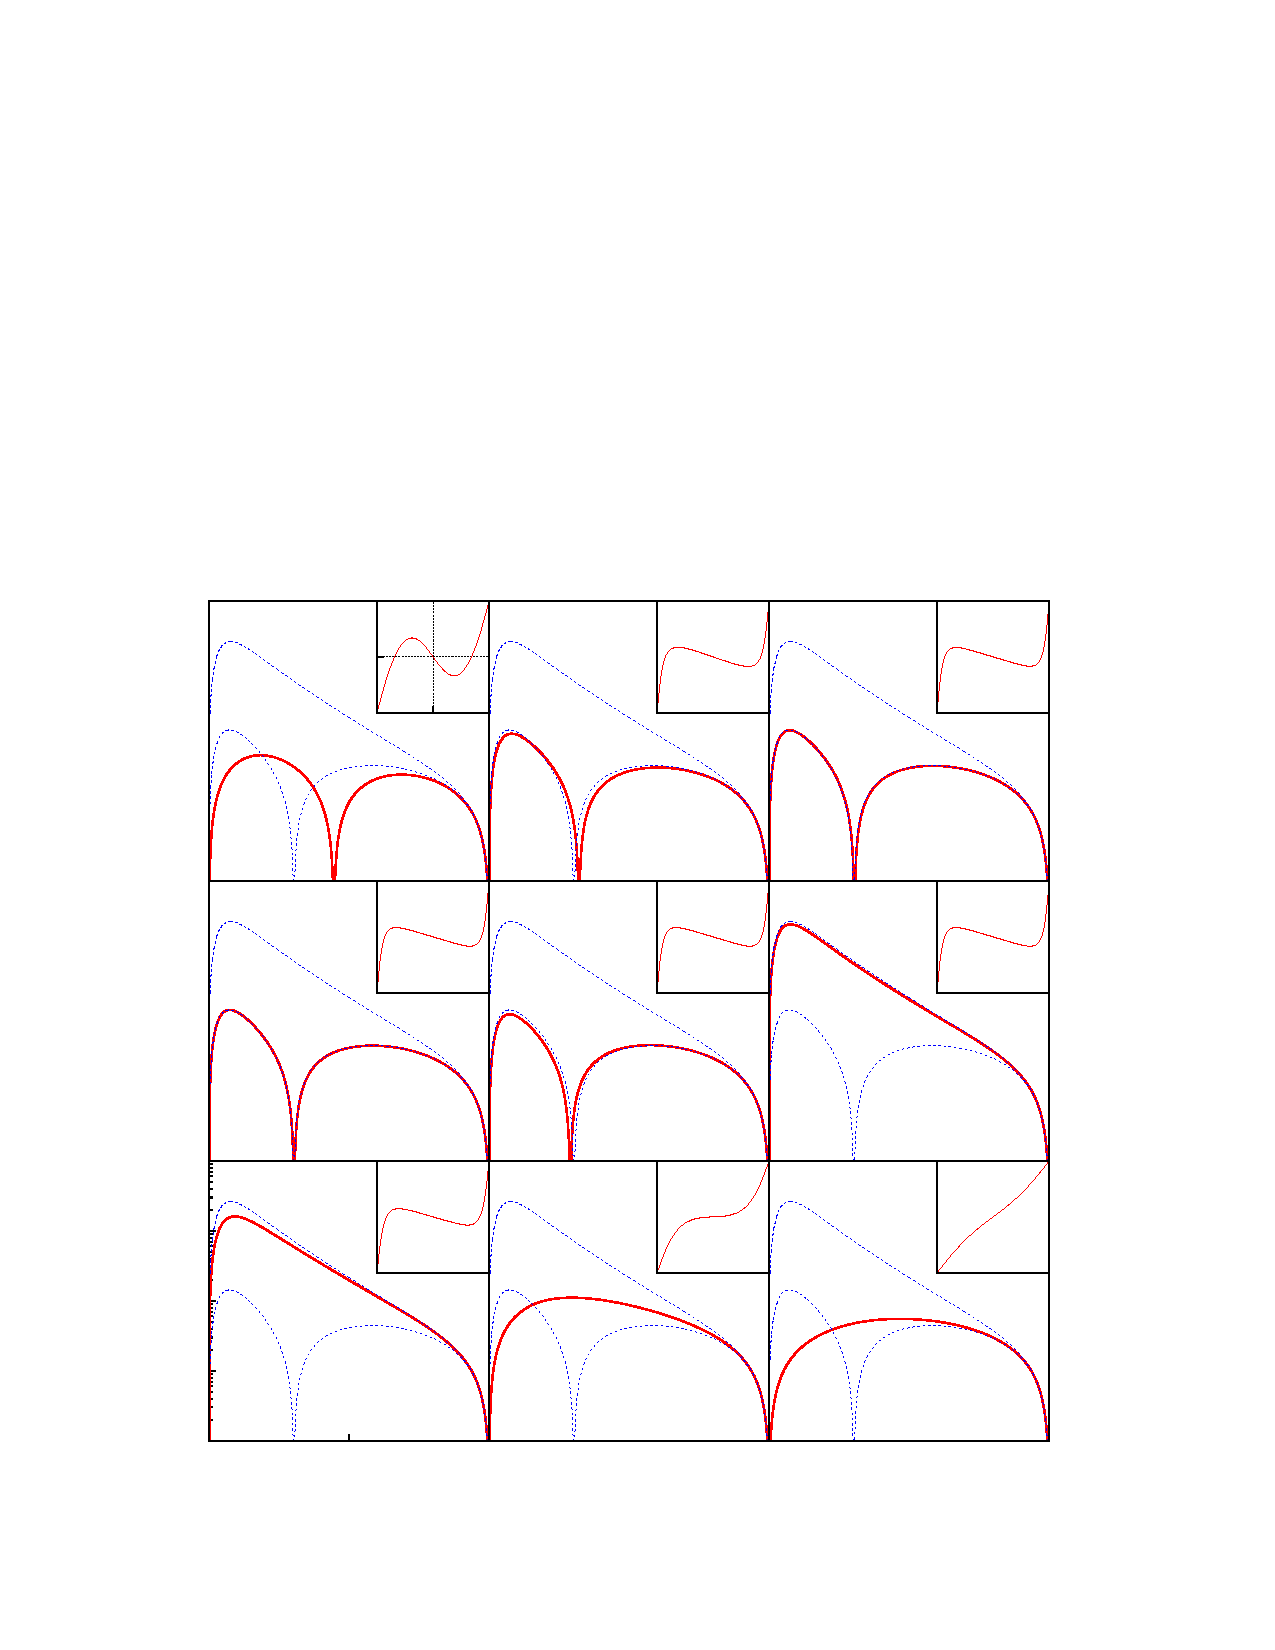
\includegraphics{graphics/snapshot_to_multiplot}}%
    \gplfronttext
  \end{picture}%
\endgroup

  \caption{This figure contains a sequence of snapshots of numerical
    solutions to the gradient flow equation with initial data
    $g_-(\psi)=\psi+B^*\cdot \sin(2\psi)$ with $B^*=...$. Each
    snapshot depicts $\lvert \partial_t f\rvert$ normalized so that
    $\lvert \partial_{tr} f(t,\pi/2)\rvert=1$ along with the plot of
    $f(t)$ in the upper right corner. For comparison the first two
    modes of $f_3$ (blue dashed lines), normalized to
    $v_{1,3}^{(3)\prime}(\pi/2)=1$ have been also depicted. The
    evolution can now be divided into the following stages: ($t=0$)
    non-linear evolution, ($t=1.5-2$) linear convergence to $f_3$
    along $\vn{3}{3}$, ($t=2.5-3.$) linear divergence along
    $\vn{1}{3}$, ($t=3.5$) non-linear approach to ground state $f_1$,
    ($t\ge4$) linear convergence to $f_1$ along $\vn{1}{1}$.}
\end{figure}
    % \caption{The first six non-trivial solutions to}
    %   \eqref{eq:f_psi_EL}}
% \end{sideways}

%%% Local Variables:
%%% mode: latex
%%% TeX-master: "master"
%%% End:
